\documentclass[aspectratio=169]{beamer}

% ── Theme & Colors ──────────────────────────────────────────────────────────
\usetheme{Madrid}
\usecolortheme{default}

\definecolor{fptblue}{RGB}{30, 58, 138}
\definecolor{fptaccent}{RGB}{221, 132, 82}
\definecolor{fptgood}{RGB}{85, 168, 104}
\definecolor{fptbad}{RGB}{196, 78, 82}

\setbeamercolor{palette primary}{bg=fptblue, fg=white}
\setbeamercolor{palette secondary}{bg=fptblue!80, fg=white}
\setbeamercolor{palette tertiary}{bg=fptblue!60, fg=white}
\setbeamercolor{structure}{fg=fptblue}
\setbeamercolor{title}{fg=white, bg=fptblue}
\setbeamercolor{frametitle}{fg=white, bg=fptblue}
\setbeamercolor{block title}{bg=fptblue, fg=white}
\setbeamercolor{block body}{bg=fptblue!5}
\setbeamercolor{item}{fg=fptblue}
\setbeamercolor{alerted text}{fg=fptbad}

\setbeamertemplate{navigation symbols}{}
\setbeamertemplate{footline}{%
    \leavevmode\hbox{%
        \begin{beamercolorbox}[wd=.333\paperwidth,ht=2.5ex,dp=1ex,center]{palette primary}%
            \usebeamerfont{author in head/foot}\insertshortauthor
        \end{beamercolorbox}%
        \begin{beamercolorbox}[wd=.334\paperwidth,ht=2.5ex,dp=1ex,center]{palette secondary}%
            \usebeamerfont{title in head/foot}\insertshorttitle
        \end{beamercolorbox}%
        \begin{beamercolorbox}[wd=.333\paperwidth,ht=2.5ex,dp=1ex,right]{palette tertiary}%
            \insertframenumber{} / \inserttotalframenumber\hspace*{2ex}
        \end{beamercolorbox}%
    }%
}

% ── Packages ────────────────────────────────────────────────────────────────
\usepackage{graphicx}
\usepackage{booktabs}
\usepackage{amsmath}
\usepackage{hyperref}
\usepackage{colortbl}
\usepackage{pgfpages}
\graphicspath{{figures/}}

% ── Speaker Notes ──────────────────────────────────────────────────────────
% Uncomment the line below to show notes on a second screen during presentation
%\setbeameroption{show notes on second screen=right}
\setbeamertemplate{note page}{\pagecolor{yellow!5}\insertnote}

% ── Title ───────────────────────────────────────────────────────────────────
\title[EV Price Prediction]{Electric Vehicle Price Prediction\\in the Vietnamese Market}
\subtitle{A Web-Scraped Dataset with LLM-Assisted Feature Extraction}
\author[Hoang et al.]{Anh~D.~D.~Hoang \and Khang~H.~Tran \and Anh~N.~Vu \and Nam~N.~Trinh}
\institute[FPT University]{%
    Information Technology Specialization\\
    FPT University, Hanoi, Vietnam
}
\date{AIL301m --- March 2026}
\titlegraphic{\includegraphics[height=1.2cm]{FPT_logo}}

\begin{document}

% ════════════════════════════════════════════════════════════════════════════
    \begin{frame}
        \titlepage
    \end{frame}
    \note{Good morning/afternoon. Our project addresses EV price prediction in Vietnam---a rapidly growing market with no structured pricing dataset. We built an end-to-end pipeline from web scraping through LLM-assisted extraction to regression modeling.}

% ════════════════════════════════════════════════════════════════════════════
    \begin{frame}{Outline}
        \tableofcontents
    \end{frame}
    \note{Here is our roadmap. We will cover motivation, data collection, the three critical data quality issues we discovered, feature engineering, model results, and our key finding about data quality versus model selection.}

% ════════════════════════════════════════════════════════════════════════════


    \section{Introduction}

    \begin{frame}{Motivation}
        \begin{columns}[T]
            \begin{column}{0.55\textwidth}
                \begin{itemize}
                    \item Vietnam's EV market is \textbf{growing rapidly}
                    \begin{itemize}
                        \item VinFast mass-producing since 2022
                        \item Chinese imports (BYD, Wuling, Geely)
                        \item Government ICE phase-out by 2040
                    \end{itemize}
                    \item \textbf{No structured dataset} exists for Vietnamese EV prices
                    \item No local equivalent of Kelley Blue Book or AutoTrader
                    \item Listings are \textbf{unstructured, Vietnamese-language}, scattered across multiple platforms
                \end{itemize}
            \end{column}
            \begin{column}{0.42\textwidth}
                \begin{block}{Gap}
                    Existing car price prediction studies rely on clean, single-source, Western-market datasets
                \end{block}
                \vspace{0.5em}
                \begin{block}{Our Goal}
                    End-to-end pipeline: \textbf{scraping $\to$ LLM extraction $\to$ data quality $\to$ prediction}
                \end{block}
            \end{column}
        \end{columns}
    \end{frame}
    \note{Vietnam's EV market is expanding fast---VinFast has been mass-producing since 2022, and Chinese brands like BYD are entering. The government plans to phase out ICE vehicles by 2040. But unlike Western markets with Kelley Blue Book or AutoTrader, there is no structured pricing dataset for Vietnamese EVs. Listings are scattered across multiple Vietnamese-language platforms with inconsistent formats. Our goal is to build the full pipeline: scraping, LLM extraction, data quality analysis, and price prediction.}

    \begin{frame}{Contributions}
        \begin{enumerate}
            \item \textbf{First Vietnamese EV dataset} --- 4,166 records from 4 marketplaces with unified 20-column schema
            \item \textbf{Two-stage LLM extraction} --- local Qwen 2.5 3B + cloud GPT-5-nano with auto-retry and Pydantic validation
            \item \textbf{Data quality analysis} --- identified and corrected 3 critical issues, reducing RMSE by \textbf{67\%} (1.02B $\to$ 332M VND)
            \item \textbf{Segment-specific evaluation} --- practical accuracy (RMSE $< 100$M) for budget \& mid-range segments (92\% of test records)
        \end{enumerate}

        \vspace{1em}
        \begin{alertblock}{Key Finding}
            Data quality remediation contributes \textbf{far more} to accuracy than model selection (67\% vs 15\% RMSE improvement).
        \end{alertblock}
    \end{frame}
    \note{We make four contributions. First, we created the first Vietnamese EV dataset---4,166 records from four marketplaces unified into a 20-column schema. Second, we used a two-stage LLM pipeline: a local Qwen 2.5 3B model for initial extraction, with GPT-5-nano for cloud verification of low-confidence records. Third---and this is our key insight---we found that fixing three data quality issues reduced RMSE by 67\%, computed as $(1.02\text{B} - 0.332\text{B}) / 1.02\text{B} = 67\%$. Fourth, our best model achieves practical accuracy for 92\% of test records, meaning RMSE under 100 million VND for budget and mid-range segments---that is 555 out of 603 test records.}

% ════════════════════════════════════════════════════════════════════════════


    \section{Data Collection}

    \begin{frame}{Data Sources}
        \begin{columns}[T]
            \begin{column}{0.55\textwidth}
                \begin{table}
                    \centering
                    \small
                    \begin{tabular}{llr}
                        \toprule
                        \textbf{Website}  & \textbf{Method} & \textbf{Records} \\
                        \midrule
                        bonbanh.com       & BeautifulSoup   & 1,493            \\
                        chotot.com        & Scrapy          & 1,666            \\
                        xevinfastluot.com & Selenium        & 279              \\
                        otodien.vn        & BeautifulSoup   & 728              \\
                        \midrule
                        \textbf{Total}    &                 & \textbf{4,166}   \\
                        \bottomrule
                    \end{tabular}
                \end{table}
                \vspace{0.5em}
                \small
                Unified schema: 20 columns covering ID, specs, condition, metadata, and price
            \end{column}
            \begin{column}{0.42\textwidth}
                \begin{figure}
                    \centering
                    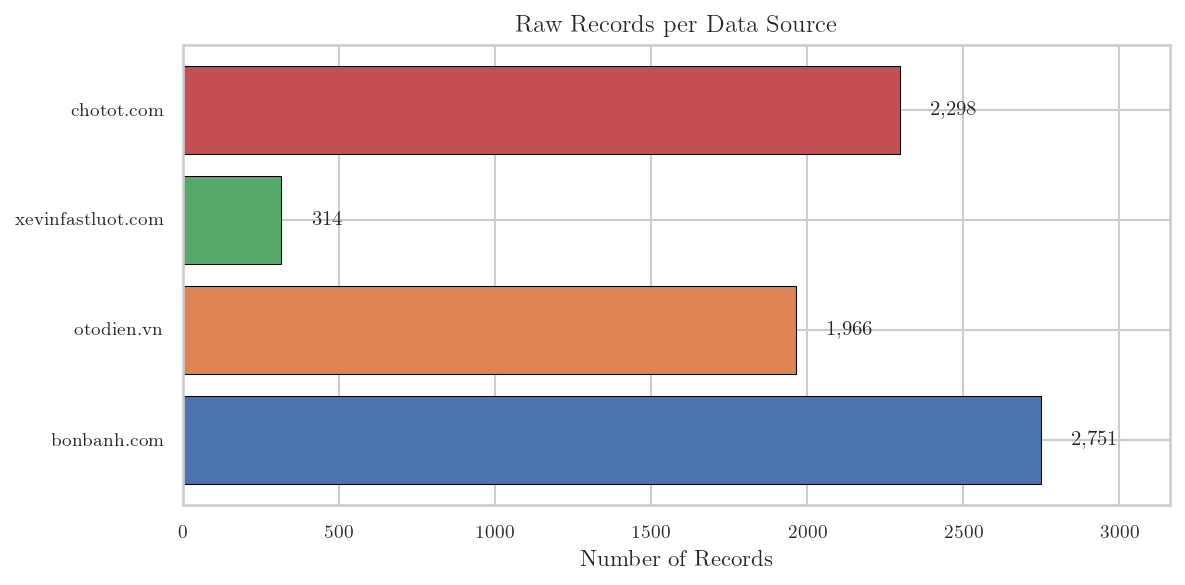
\includegraphics[width=\textwidth]{records_per_source}
                    \caption{Records per source}
                \end{figure}
            \end{column}
        \end{columns}
    \end{frame}
    \note{We scraped four Vietnamese EV marketplaces using different techniques depending on each site's structure. bonbanh.com and otodien.vn use server-rendered HTML, so BeautifulSoup was sufficient. chotot.com loads data via API, so we used Scrapy. xevinfastluot.com uses JavaScript rendering, requiring Selenium. In total we collected 4,166 records, unified into a common 20-column schema covering ID, specs, condition, metadata, and price.}

    \begin{frame}{LLM-Assisted Feature Extraction}
        \begin{block}{Two-Stage Pipeline}
            \begin{enumerate}
                \item \textbf{Local --- Qwen 2.5 3B} (via Ollama)
                \begin{itemize}
                    \item Zero-shot prompt $\to$ JSON output
                    \item Pydantic schema validation
                    \item Auto-retry up to 3 attempts on failure
                \end{itemize}
                \item \textbf{Cloud --- GPT-5-nano} (verification)
                \begin{itemize}
                    \item Batch-processes low-confidence records
                    \item Corrects hallucinated trim names
                \end{itemize}
            \end{enumerate}
        \end{block}

        \vspace{0.5em}
        \begin{columns}[T]
            \begin{column}{0.45\textwidth}
                \textbf{Fill rates:}\\[0.3em]
                \small
                Brand: 99.3\% \quad Base model: 98.7\%\\
                Year: 98.3\% \quad Price: 100\%
            \end{column}
            \begin{column}{0.45\textwidth}
                \textbf{Failure mode:}\\[0.3em]
                \small
                Trim-level hallucination for non-VinFast brands
            \end{column}
        \end{columns}
    \end{frame}
    \note{Raw listing text is unstructured Vietnamese. We used a two-stage LLM pipeline to extract structured fields. Stage one: a local Qwen 2.5 3B model running via Ollama processes each listing with a zero-shot prompt, returning JSON validated against a Pydantic schema. If validation fails, we auto-retry up to 3 times. Stage two: records where the local model had low confidence are batch-processed by GPT-5-nano in the cloud, which corrects issues like hallucinated trim names for non-VinFast brands. Fill rates were high: brand at 99.3\%, base model at 98.7\%, year at 98.3\%, and price at 100\%.}

% ════════════════════════════════════════════════════════════════════════════


    \section{Data Quality Analysis}

    \begin{frame}{Three Critical Issues}
        \begin{columns}[T]
            \begin{column}{0.32\textwidth}
                \begin{block}{\small 1. chotot.com 10$\times$ Inflation}
                    \small
                    \begin{itemize}
                        \item 1,666 records (40\%)
                        \item chotot.com prices stored in 1,000~VND units
                        \item Fix: divide by 10
                    \end{itemize}
                \end{block}
            \end{column}
            \begin{column}{0.32\textwidth}
                \begin{block}{\small 2. BYD Pricing Error}
                    \small
                    \begin{itemize}
                        \item 90 records (2.3\%)
                        \item $\sim$56\% of total weighted error
                        \item Fix: remove all BYD
                    \end{itemize}
                \end{block}
            \end{column}
            \begin{column}{0.32\textwidth}
                \begin{block}{\small 3. Duplicate Leakage}
                    \small
                    \begin{itemize}
                        \item 887 duplicates (22\%)
                        \item Inflated $R^2$: 0.787
                        \item Honest $R^2$: 0.725
                    \end{itemize}
                \end{block}
            \end{column}
        \end{columns}

        \vspace{1em}
        \centering
        \begin{tabular}{lrr}
            \toprule
            \textbf{Stage}      & \textbf{Records} & \textbf{Best RMSE} \\
            \midrule
            Raw (all issues)    & 3,992            & 1.02B VND          \\
            + All fixes applied & 3,015            & \textbf{332M VND}  \\
            \bottomrule
        \end{tabular}
        \quad \textcolor{fptgood}{\textbf{$\downarrow$ 67\% RMSE reduction}}
    \end{frame}
    \note{This is the most important slide. We discovered three critical issues in the scraped data.

    \textbf{First:} chotot.com stores prices in units of 1,000 VND, but our scraper ingested them as raw VND---making all 1,666 chotot records appear 10 times more expensive. That is 40\% of our data. We detected this by comparing the same car models across sources---for example, a VF5 Plus 2024 showed 3.99 billion on chotot versus 399 million on bonbanh. The fix was simply dividing chotot prices by 10.

    \textbf{Second:} All 90 BYD records---2.3\% of the data---had systematically wrong prices. We simulated the error by comparing listed prices against known MSRPs for Atto 3, Dolphin, and M6 models. The simulated mean absolute error for BYD was 4.914 billion VND per record, versus just 89.5 million for non-BYD records from our Random Forest model. We measured contribution using weighted error: $\frac{\text{BYD MAE} \times n_{\text{BYD}}}{\text{BYD MAE} \times n_{\text{BYD}} + \text{RF MAE} \times n_{\text{non-BYD}}} \approx 56\%$. So BYD accounts for roughly 56\% of total prediction error despite being only 2.3\% of records. We removed all BYD records.

    \textbf{Third:} 887 records---22.2\% of the cleaned dataset---were exact duplicates. We detected duplicates by matching on 7 columns: brand, base\_model, model\_mode, year, price, condition, and mileage, using pandas duplicated with keep=first. The most extreme case was a VinFast VF9 2025 at 12.29 billion appearing 23 times. These duplicates leaked between train and test sets, inflating our $R^2$. We derived the inflation mathematically: $\text{SS}_{\text{res}} = \text{RMSE}^2 \times n_{\text{test}}$, then $\text{Var}(y) = \frac{\text{SS}_{\text{res}}}{(1 - R^2) \times n_{\text{test}}}$. With 177 extra duplicate test records (20\% of 887), inflated $R^2 = 1 - \frac{\text{SS}_{\text{res}}}{\text{Var}(y) \times n_{\text{inflated}}} = 0.787$. Honest $R^2$ after dedup is 0.725---a 6.2 percentage point inflation.

    The bottom line: fixing all three issues took RMSE from 1.02 billion down to 332 million---a 67\% reduction.}

    \begin{frame}{chotot.com Price Inflation}
        \begin{figure}
            \centering
            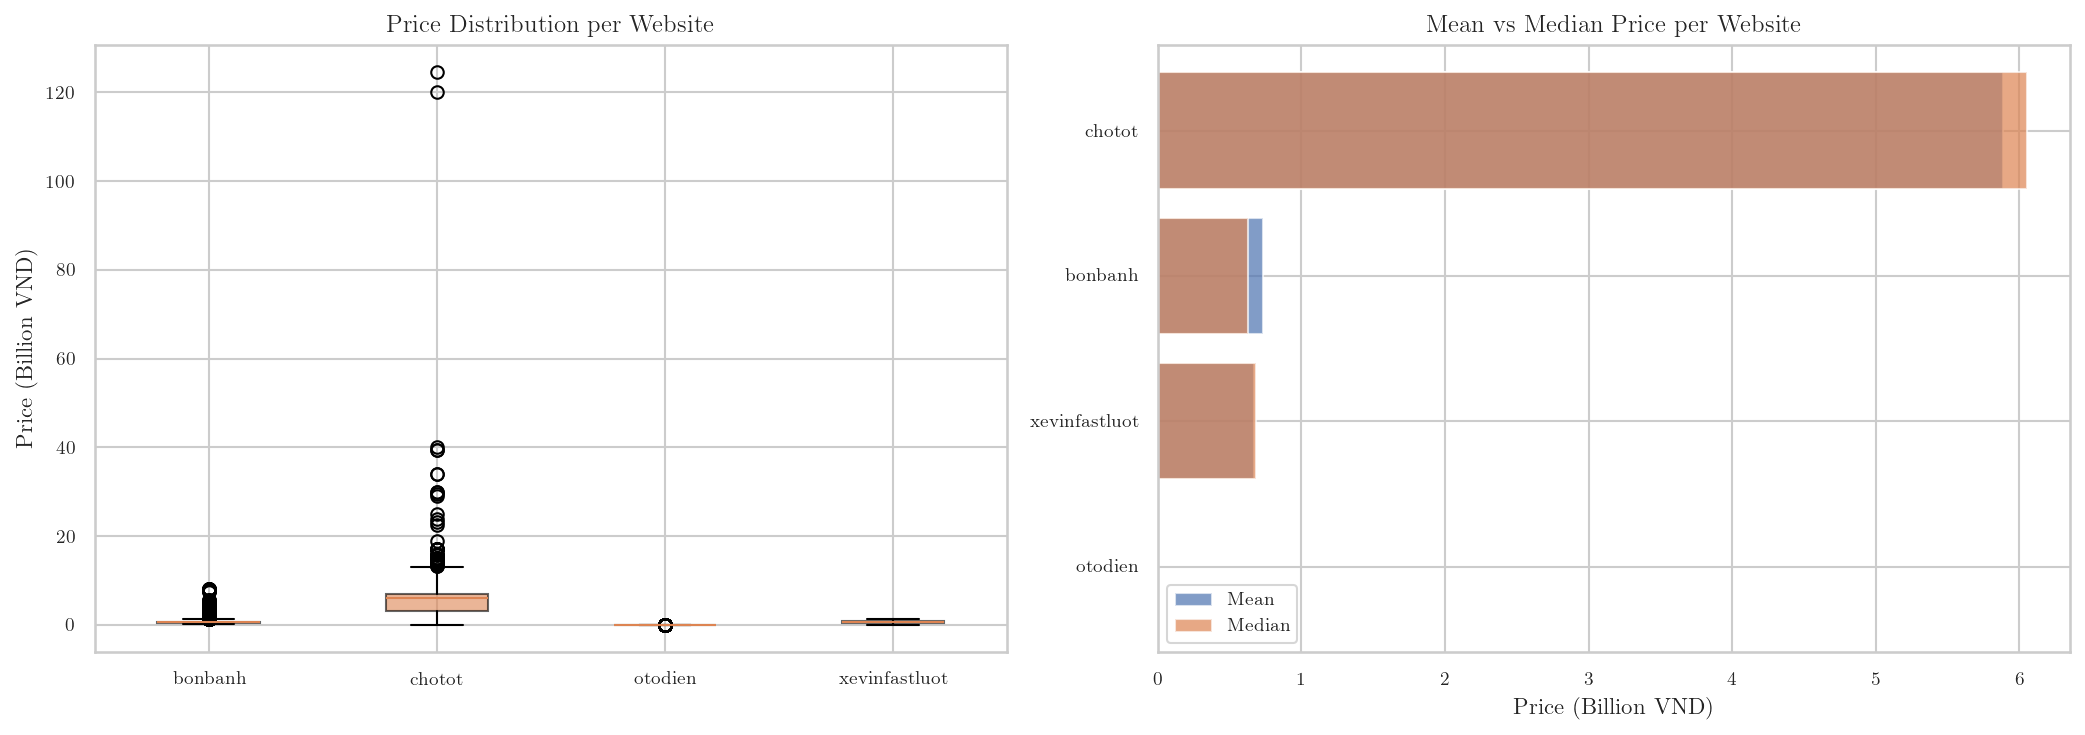
\includegraphics[width=0.85\textwidth]{chotot_price_comparison}
            \caption{Systematic 10$\times$ price inflation from chotot.com vs other sources}
        \end{figure}
    \end{frame}
    \note{This figure shows the systematic 10x inflation visually. Each group is a car model. The orange bars---chotot prices---are consistently about 10 times higher than the blue bars from other sources. This pattern made detection straightforward once we compared across sources. For example, a VF5 Plus 2024 shows 3.99 billion VND on chotot versus 399 million on bonbanh---exactly a factor of 10.}

    \begin{frame}{Before vs After Data Quality Fixes}
        \begin{figure}
            \centering
            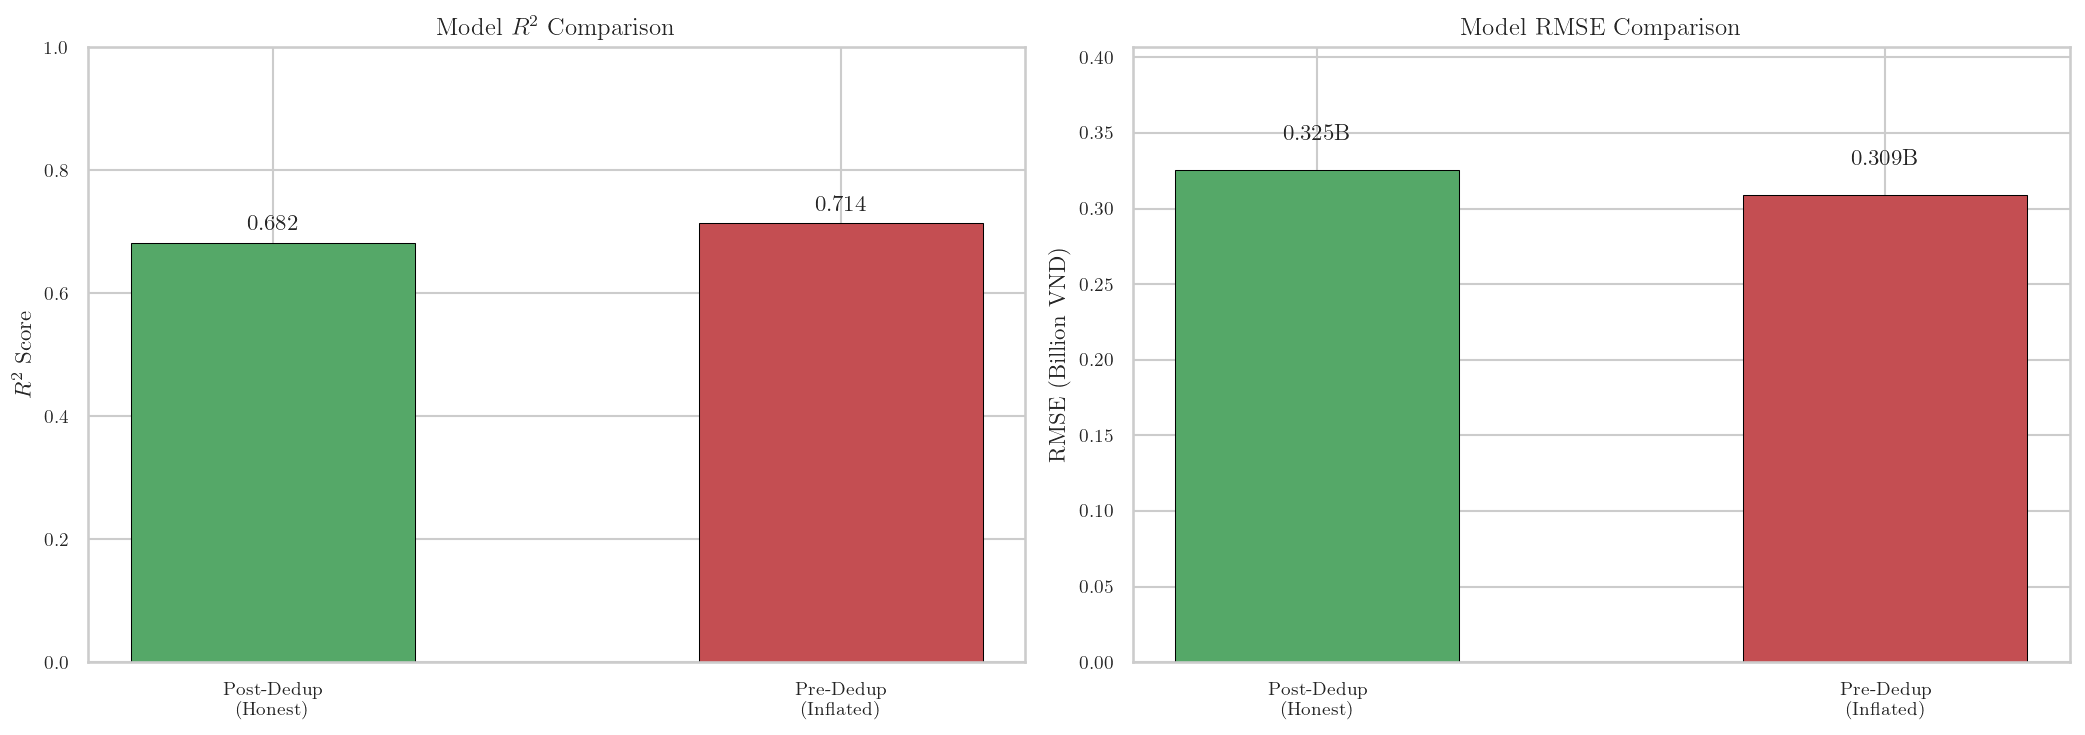
\includegraphics[width=0.85\textwidth]{before_after_comparison}
            \caption{Model performance before and after corrections --- ``before'' metrics were inflated by leakage}
        \end{figure}
    \end{frame}
    \note{This three-panel figure compares model performance before and after our corrections. Important caveat: the ``before'' metrics were inflated by duplicate leakage between train and test sets. When the same record appears in both sets, the model essentially memorizes it, producing near-zero error on those test points---this is a form of data leakage.

    How we measured test-train overlap: we detected duplicates by matching on 7 columns (brand, base\_model, model\_mode, year, price, condition, mileage). With an 80/20 random split, approximately 20\% of the 887 duplicates---about 177 records---would appear in the test set with matching copies in the training set, giving the model ``free'' correct answers.

    The ``after'' metrics reflect honest evaluation on deduplicated, price-corrected data. All four models improved dramatically---Random Forest RMSE dropped from over 1 billion to 332 million VND.}

% ════════════════════════════════════════════════════════════════════════════


    \section{Feature Engineering}

    \begin{frame}{Feature Engineering Pipeline}
        \begin{columns}[T]
            \begin{column}{0.48\textwidth}
                \textbf{41 features} from 3,015 records:
                \vspace{0.5em}
                \small
                \begin{tabular}{lr}
                    \toprule
                    \textbf{Category}              & \textbf{Count} \\
                    \midrule
                    Numeric (age, mileage, \ldots) & 4              \\
                    EV Specs (kWh, range, hp)      & 3              \\
                    Target-encoded                 & 2              \\
                    One-hot (brand, model, \ldots) & 32             \\
                    \midrule
                    \textbf{Total}                 & \textbf{41}    \\
                    \bottomrule
                \end{tabular}
            \end{column}
            \begin{column}{0.48\textwidth}
                \begin{block}{Key Decisions}
                    \begin{itemize}
                        \small
                        \item \textbf{EV specs recovery}: battery, range, power from otodien.vn lookup (29 models)
                        \item \textbf{Hybrid encoding}: target-encode only high-cardinality features
                        \item Target-encoding everything $\Rightarrow$ $R^2$ drops to 0.087!
                    \end{itemize}
                \end{block}
            \end{column}
        \end{columns}
    \end{frame}
    \note{From the cleaned 3,015 records, we engineered 41 features in three categories. Four numeric features: vehicle age, mileage, and two derived. Three EV-specific features: battery capacity in kWh, range in km, and power in horsepower---these were recovered by joining with a lookup table from otodien.vn covering 29 EV models. Two target-encoded features for high-cardinality categorical columns like base\_model. And 32 one-hot encoded features for lower-cardinality categories.

    A key decision: we only target-encode high-cardinality features. Target encoding uses leave-one-out encoding with Bayesian smoothing ($m=10$) to prevent overfitting---it replaces each category with the mean target value of other records with the same category, smoothed toward the global mean. When we tried target-encoding everything, $R^2$ collapsed to 0.087---basically no predictive power---because low-cardinality features lost too much categorical signal.}

    \begin{frame}{EV Specifications Recovery}
        \begin{figure}
            \centering
            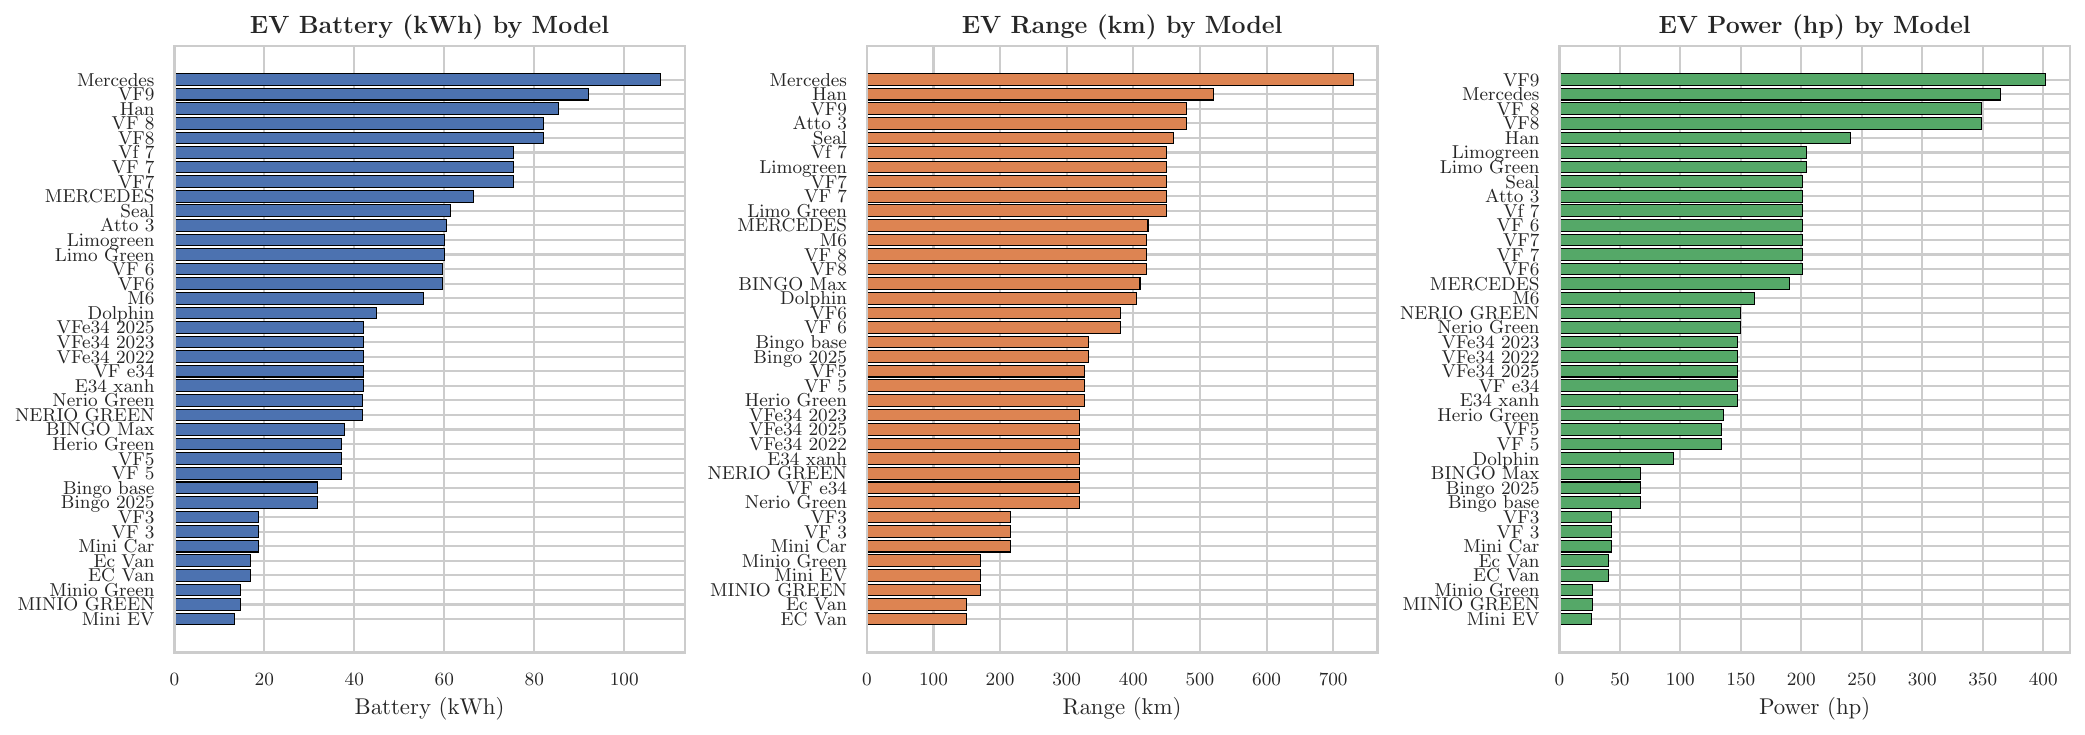
\includegraphics[width=0.85\textwidth]{ev_specs_coverage}
            \caption{EV specifications across models --- captures fundamental pricing physics}
        \end{figure}
    \end{frame}
    \note{This figure shows the coverage of EV specifications across car models. Battery capacity, range, and power capture fundamental pricing physics---a car's range and performance directly determine its value. We recovered these from otodien.vn's specification pages for 29 EV models, then joined them to our main dataset by brand and model. The lookup table was built by scraping otodien.vn's 728 records which include detailed spec fields that other sources lack.}

    \begin{frame}{Encoding Strategy \& Feature Importance}
        \begin{columns}[T]
            \begin{column}{0.45\textwidth}
                \begin{figure}
                    \centering
                    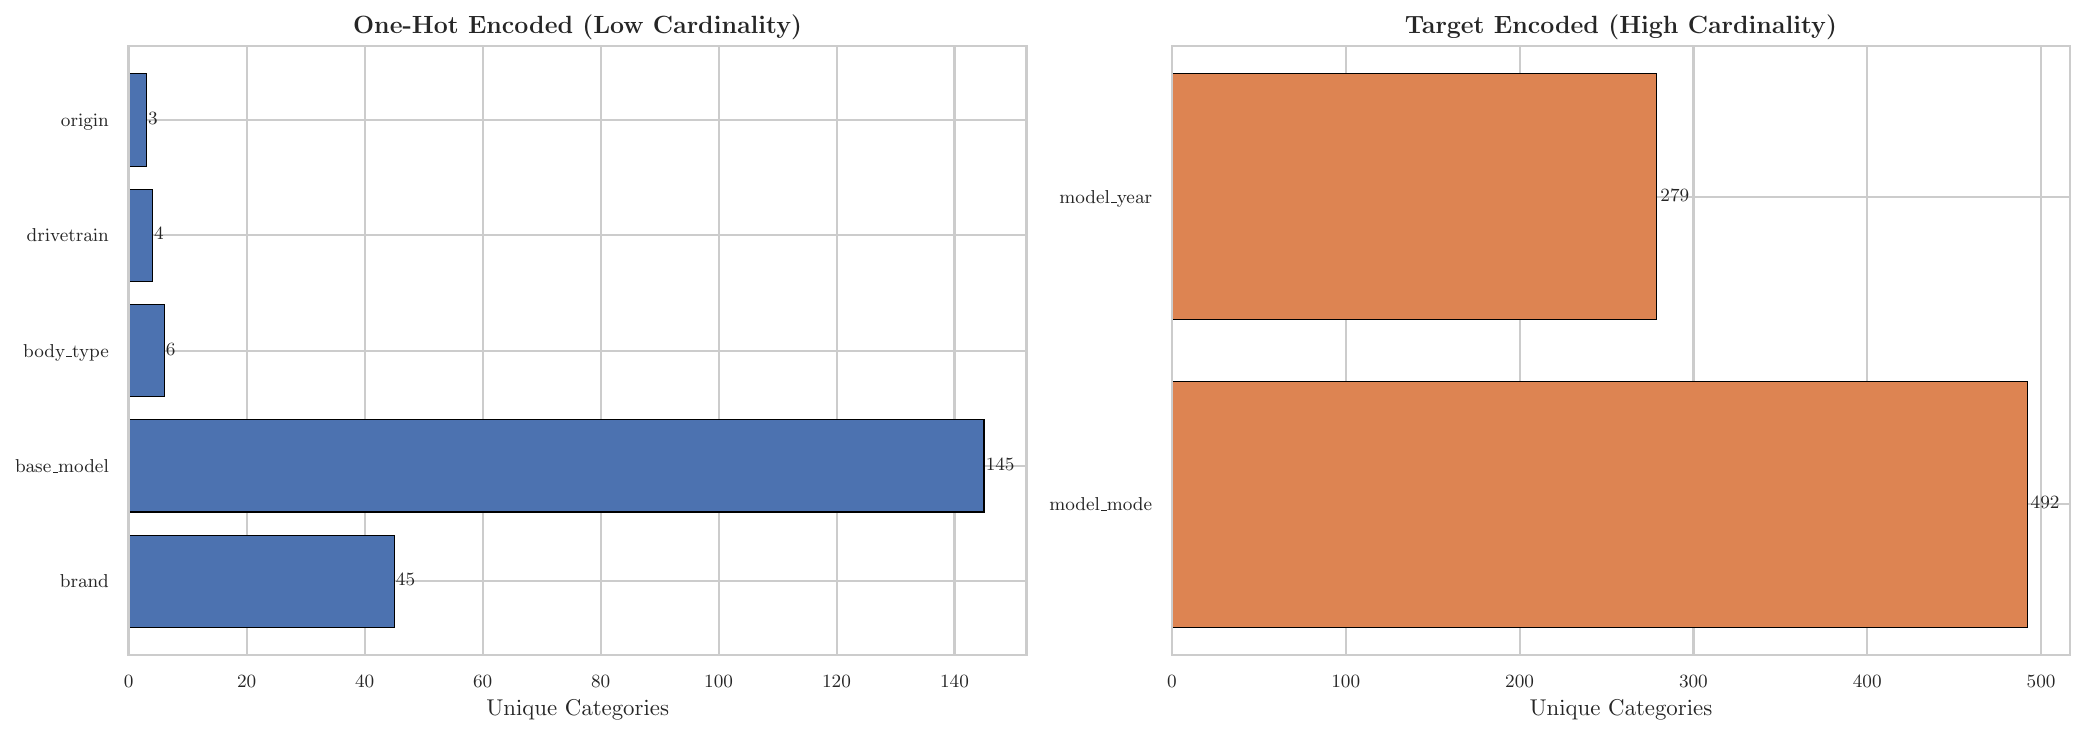
\includegraphics[width=\textwidth]{encoding_comparison}
                    \caption{Hybrid encoding}
                \end{figure}
            \end{column}
            \begin{column}{0.52\textwidth}
                \begin{figure}
                    \centering
                    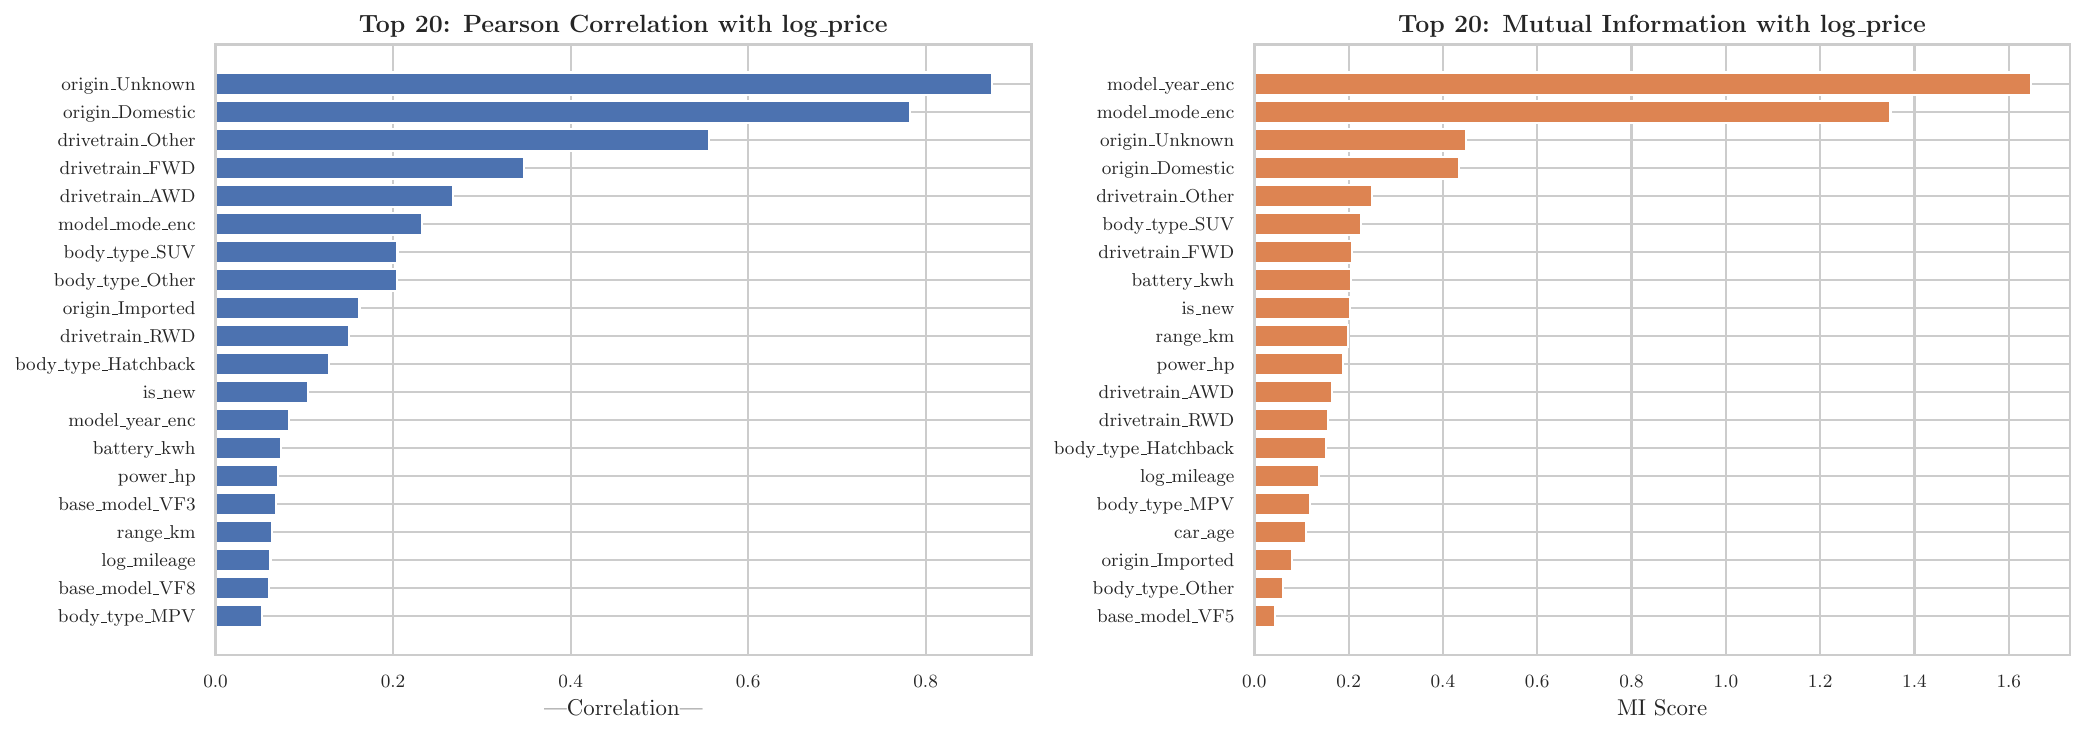
\includegraphics[width=\textwidth]{feature_importance_summary}
                    \caption{Top features by correlation \& MI}
                \end{figure}
            \end{column}
        \end{columns}
    \end{frame}
    \note{On the left, the encoding comparison shows why hybrid encoding outperforms pure target encoding. On the right, we see the top features ranked by two measures: Pearson correlation with price, which captures linear relationships, and mutual information (MI) which captures non-linear dependencies. MI is estimated using $k$-nearest-neighbor distances and measures how much knowing a feature reduces uncertainty about the target.

    The model\_mode feature has the highest Pearson correlation---$r = 0.76$ with price. EV specs like battery\_kwh and range\_km rank high on mutual information, confirming they capture non-linear pricing relationships that correlation alone misses. For example, battery capacity may have a threshold effect where larger batteries command disproportionately higher prices.}

% ════════════════════════════════════════════════════════════════════════════


    \section{Experimental Setup}

    \begin{frame}{Experimental Setup}
        \begin{columns}[T]
            \begin{column}{0.48\textwidth}
                \textbf{Data Split:}
                \begin{itemize}
                    \item 80/20 train--test (2,412 / 603)
                    \item Stratified on \texttt{base\_model}
                    \item Sample weights: inverse quintile frequency
                \end{itemize}

                \vspace{1em}
                \textbf{Evaluation:}
                \begin{itemize}
                    \item RMSE, MAE, $R^2$, Adj.\ $R^2$, MAPE
                    \item 95\% CI via bootstrap (1,000 resamples)
                    \item Segment-specific analysis
                \end{itemize}
            \end{column}
            \begin{column}{0.48\textwidth}
                \textbf{Four Models:}
                \vspace{0.5em}
                \small
                \begin{tabular}{ll}
                    \toprule
                    \textbf{Model} & \textbf{Input}      \\
                    \midrule
                    Ridge          & Scaled + log target \\
                    SVR (RBF)      & Scaled + log target \\
                    Random Forest  & Raw features        \\
                    XGBoost        & Raw features        \\
                    \bottomrule
                \end{tabular}

                \vspace{1em}
                \normalsize
                All tuned via \textbf{5-fold CV} with GridSearchCV
            \end{column}
        \end{columns}
    \end{frame}
    \note{Our setup: 80/20 train-test split---2,412 training, 603 test records---stratified on base\_model so each car model's proportion is preserved in both sets. Models with fewer than 5 records were grouped into a ``\_rare\_'' stratum to ensure valid stratification.

    We trained four models: Ridge and SVR with StandardScaler-normalized features and log-transformed target ($\log(1+y)$), Random Forest and XGBoost with raw features. All were tuned via 5-fold cross-validation using GridSearchCV with negative mean squared error as the scoring metric---this means the model that minimizes prediction error on held-out folds wins.

    For evaluation, we report five metrics on the held-out test set: RMSE (root mean squared error, penalizes large errors), MAE (mean absolute error, robust to outliers), $R^2$ (fraction of variance explained), adjusted $R^2$ (corrected for number of features), and MAPE (mean absolute percentage error). We also compute 95\% confidence intervals via bootstrap resampling---drawing 1,000 random samples with replacement from the test predictions, computing RMSE for each sample, then taking the 2.5th and 97.5th percentiles as bounds.}

% ════════════════════════════════════════════════════════════════════════════


    \section{Results}

    \begin{frame}{Overall Benchmark}
        \begin{table}
            \centering
            \begin{tabular}{lrrrrr}
                \toprule
                \textbf{Model}                               & \textbf{RMSE} & \textbf{MAE} & $\boldsymbol{R^2}$ & \textbf{Adj.\ $R^2$} & \textbf{MAPE} \\
                & (M VND)       & (M VND)      &                    &                      & (\%)          \\
                \midrule
                Ridge                                        & 381           & 115          & 0.636              & 0.610                & 43.5          \\
                SVR                                          & 369           & 94           & 0.660              & 0.635                & 48.9          \\
                \rowcolor{fptblue!10} \textbf{Random Forest} & \textbf{332}  & \textbf{89}  & \textbf{0.725} & \textbf{0.705} & \textbf{43.6} \\
                XGBoost                                      & 383           & 103          & 0.633              & 0.606                & 43.0          \\
                \bottomrule
            \end{tabular}
            \caption{Test set results ($n = 603$). RF 95\% CI for RMSE: [139M, 496M] VND.}
        \end{table}

        \vspace{0.5em}
        \centering
        \textcolor{fptblue}{\textbf{Random Forest wins across all metrics}}
    \end{frame}
    \note{Here are the results. Random Forest wins across all metrics: RMSE of 332 million, MAE of 89 million, $R^2$ of 0.725. The 95\% bootstrap confidence interval for RF RMSE is 139 to 496 million VND---the wide range reflects high variance from luxury outliers pulling up RMSE in some bootstrap samples.

    Notice the models are relatively close---the gap between best (RF at 332M) and worst (XGBoost at 383M) is only 51 million, or about 15\%. This 15\% is computed as $(383 - 332) / 332 = 15.4\%$. This supports our thesis that data quality matters more than model choice.}

    \begin{frame}{Model Comparison}
        \begin{columns}[c]
            \begin{column}{0.48\textwidth}
                \begin{figure}
                    \centering
                    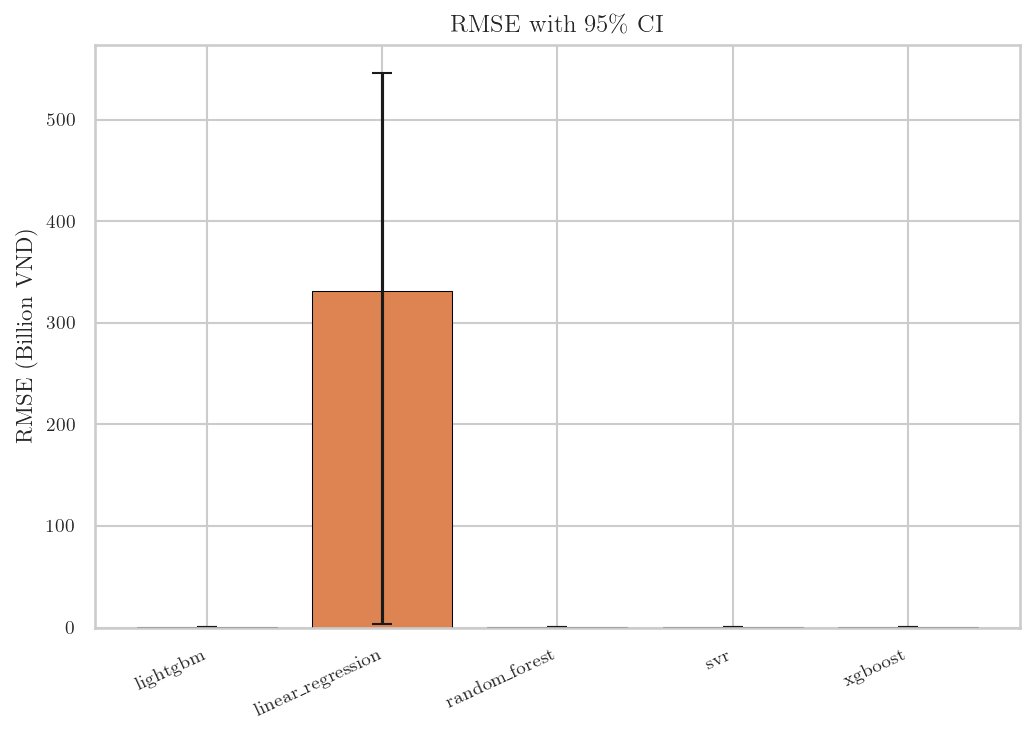
\includegraphics[width=\textwidth]{model_rmse_comparison}
                    \caption{RMSE comparison}
                \end{figure}
            \end{column}
            \begin{column}{0.48\textwidth}
                \begin{figure}
                    \centering
                    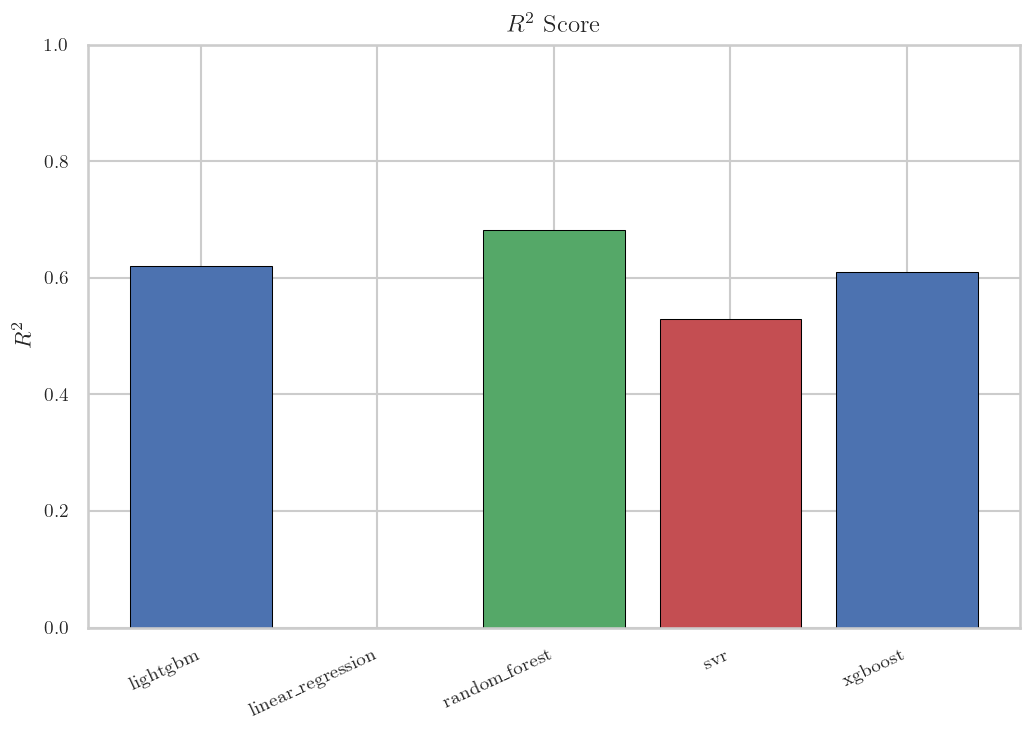
\includegraphics[width=\textwidth]{model_r2_comparison}
                    \caption{$R^2$ comparison}
                \end{figure}
            \end{column}
        \end{columns}
    \end{frame}
    \note{These bar charts visualize the benchmark table. Left panel shows RMSE---lower is better---with Random Forest clearly leading. Right panel shows $R^2$---higher is better---again RF on top at 0.725. The visual makes the 15\% gap between models apparent, but also shows it is relatively small compared to the 67\% improvement from data cleaning.}

    \begin{frame}{Segment-Specific Performance}
        \begin{columns}[T]
            \begin{column}{0.45\textwidth}
                \begin{table}
                    \centering
                    \small
                    \begin{tabular}{lrr}
                        \toprule
                        \textbf{Segment}  & \textbf{RMSE}               & $\boldsymbol{n}$ \\
                        \midrule
                        Budget ($<$500M)  & \textcolor{fptgood}{100M}   & 237              \\
                        Mid (0.5--1.2B)   & \textcolor{fptgood}{81M}    & 318              \\
                        Premium (1.2--5B) & \textcolor{fptaccent}{797M} & 46               \\
                        Luxury ($>$5B)    & \textcolor{fptbad}{4,041M}  & 2                \\
                        \midrule
                        \textbf{Overall}  & \textbf{332M}               & 603              \\
                        \bottomrule
                    \end{tabular}
                    \caption{RF by segment}
                \end{table}
                \vspace{0.3em}
                \small
                Budget + Mid = \textbf{92\% of test data} with practical RMSE
            \end{column}
            \begin{column}{0.52\textwidth}
                \begin{figure}
                    \centering
                    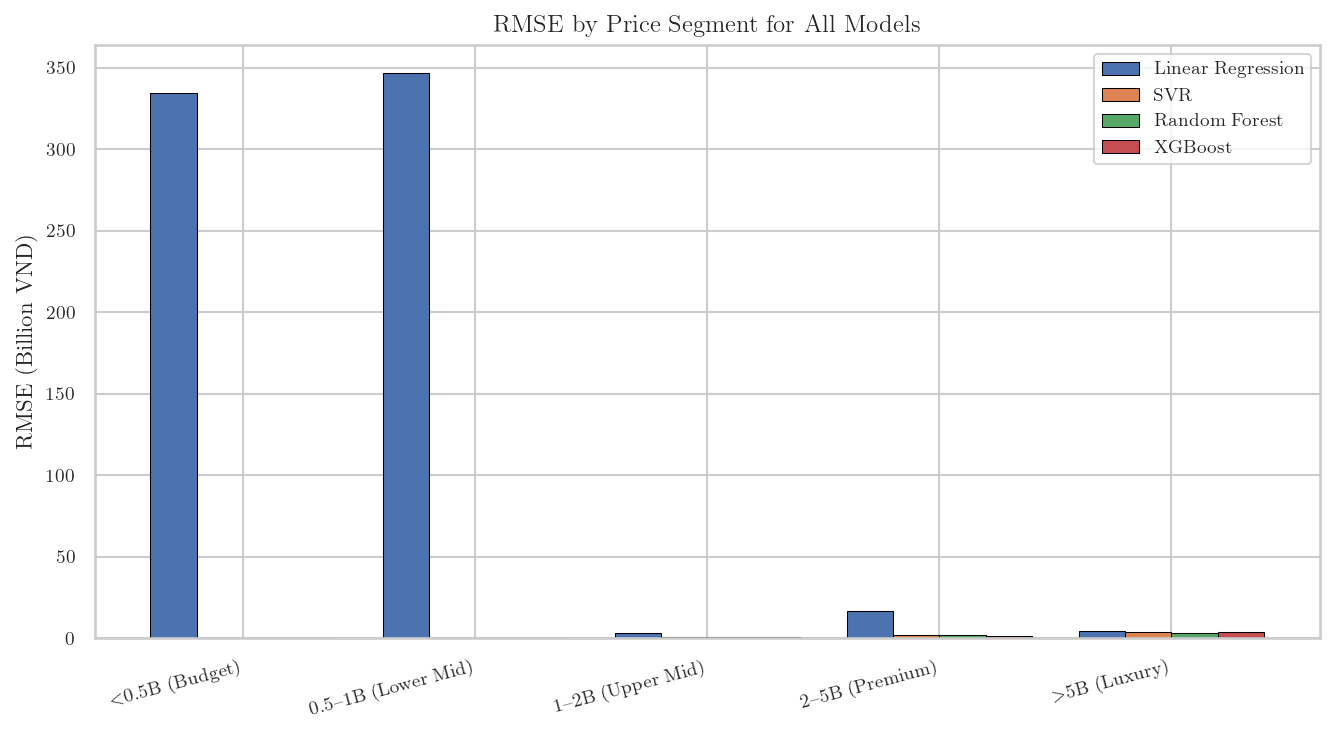
\includegraphics[width=\textwidth]{segment_rmse}
                    \caption{RMSE by segment (all models)}
                \end{figure}
            \end{column}
        \end{columns}
    \end{frame}
    \note{This is where it gets practical. We divided the test set into four price segments: budget under 500 million, mid-range 500M to 1.2 billion, premium 1.2B to 5B, and luxury above 5 billion. Segment boundaries were chosen based on the Vietnamese EV market price distribution.

    Budget segment: 237 test records, RMSE of 100 million---that is 34\% of the median budget car price. We computed this as $\text{RMSE}_{\text{segment}} / \text{median}(y_{\text{segment}})$, so $100\text{M} / 293\text{M} \approx 34\%$. Mid-range: 318 records, RMSE of 81 million---just 11\% of median mid-range price ($81\text{M} / 740\text{M} \approx 11\%$). These two segments together cover 555 of 603 test records---that is the 92\% figure ($555/603 = 92.0\%$). For someone buying a budget or mid-range EV, our model's error is within a practical negotiation range.

    Premium and luxury segments have much higher RMSE---797 million and 4 billion respectively---but these have far fewer records (46 and 2) and much higher price variance.}

    \begin{frame}{Random Forest: Predictions \& Feature Importance}
        \begin{columns}[c]
            \begin{column}{0.48\textwidth}
                \begin{figure}
                    \centering
                    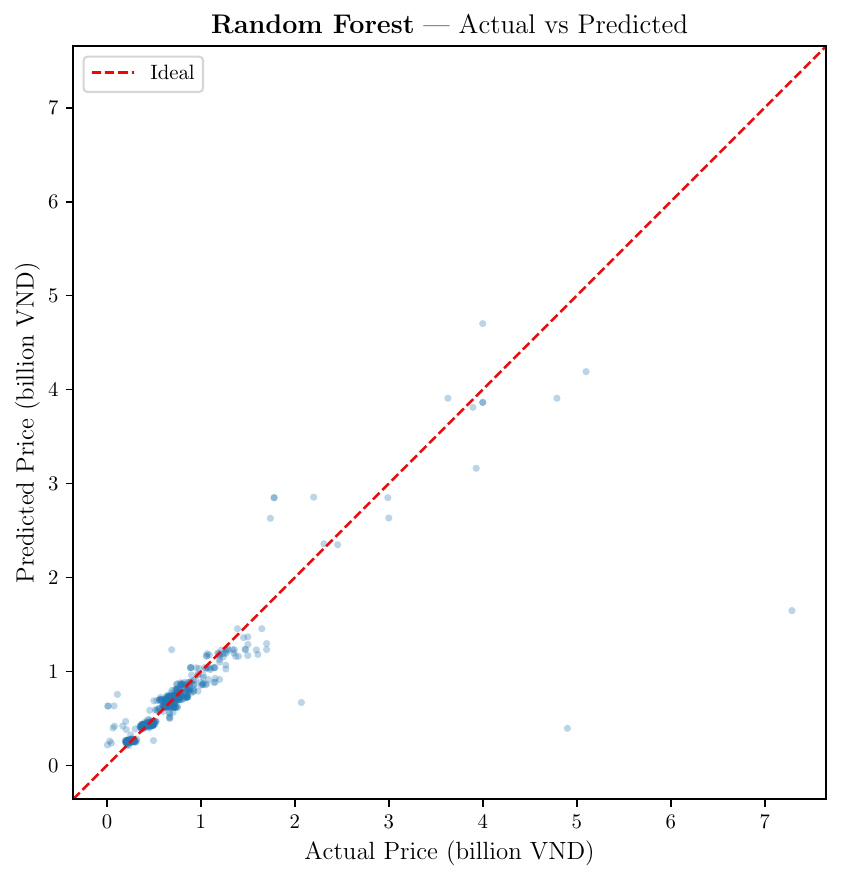
\includegraphics[width=\textwidth]{random_forest_actual_vs_predicted}
                    \caption{Actual vs Predicted}
                \end{figure}
            \end{column}
            \begin{column}{0.48\textwidth}
                \begin{figure}
                    \centering
                    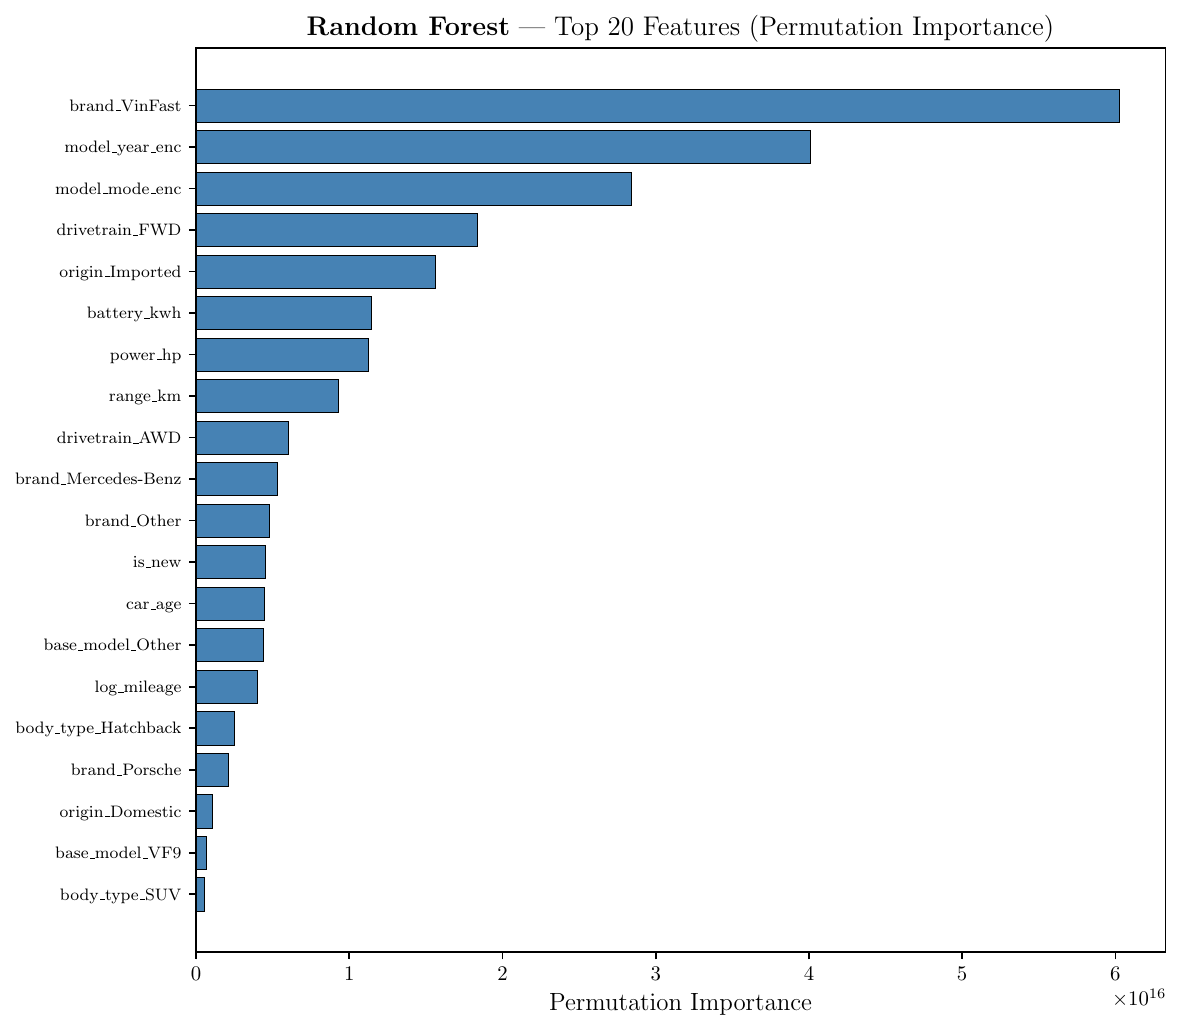
\includegraphics[width=\textwidth]{random_forest_feature_importance}
                    \caption{Top 20 feature importance}
                \end{figure}
            \end{column}
        \end{columns}
    \end{frame}
    \note{Left: actual versus predicted prices for Random Forest. Points cluster along the diagonal for budget and mid-range, confirming good predictions there. The scatter increases at higher prices---consistent with our segment analysis. The diagonal line represents perfect prediction; points below it mean the model underestimates, above it means overestimation.

    Right: the top 20 features by permutation importance---measured by randomly shuffling each feature 10 times and recording the mean increase in MSE. If shuffling a feature increases error a lot, that feature is important. model\_mode, battery\_kwh, and base\_model dominate, confirming that vehicle identity and EV specifications are the primary price drivers. This aligns with intuition: which car model you are buying and its battery/range specs are the strongest determinants of price.}

% ════════════════════════════════════════════════════════════════════════════


    \section{Discussion \& Conclusion}

    \begin{frame}{Data Quality vs Model Selection}
        \begin{columns}[T]
            \begin{column}{0.48\textwidth}
                \begin{block}{Data Quality Fixes}
                    RMSE: 1.02B $\to$ 332M VND\\
                    \textcolor{fptgood}{\textbf{$\downarrow$ 67\% improvement}}
                    \begin{itemize}
                        \small
                        \item chotot.com price correction
                        \item Deduplication (22\% removed)
                        \item BYD removal
                    \end{itemize}
                \end{block}
            \end{column}
            \begin{column}{0.48\textwidth}
                \begin{block}{Model Selection}
                    Best vs Worst: 332M vs 383M\\
                    \textcolor{fptaccent}{\textbf{$\downarrow$ 15\% difference}}
                    \begin{itemize}
                        \small
                        \item RF vs XGBoost: 51M gap
                        \item All models benefit equally from clean data
                    \end{itemize}
                \end{block}
            \end{column}
        \end{columns}

        \vspace{1em}
        \begin{alertblock}{Takeaway}
            In applied ML with web-scraped data, \textbf{invest in data quality first} --- it yields 4$\times$ more improvement than model experimentation.
        \end{alertblock}
    \end{frame}
    \note{This is our central finding. Data quality fixes---correcting chotot prices, removing duplicates, removing BYD---reduced RMSE by 67\%, from 1.02 billion to 332 million. The 67\% is $(1.02\text{B} - 0.332\text{B}) / 1.02\text{B}$. Model selection---choosing RF over XGBoost---only accounts for a 15\% difference, computed as $(383\text{M} - 332\text{M}) / 332\text{M}$, or 51 million VND.

    The ratio is roughly $67\% / 15\% \approx 4\times$. In applied machine learning with web-scraped data, the dominant bottleneck is data quality, not model architecture. This has practical implications: teams working with scraped data should invest in data validation and cross-source comparison before spending time on model experimentation. All four models benefited equally from clean data---the improvement was not model-specific.}

    \begin{frame}{Limitations \& Future Work}
        \textbf{Limitations:}
        \begin{itemize}
            \item \textbf{Brand concentration} --- VinFast = 93.6\% of records
            \item \textbf{Small dataset} --- 3,015 records (2,412 train)
            \item \textbf{No temporal modeling} --- cross-sectional only
            \item \textbf{Luxury segment} --- only 2 test records ($n$ too small)
        \end{itemize}

        \vspace{1em}
        \textbf{Future Work:}
        \begin{enumerate}
            \item Continuous scraping $\to$ time-series depreciation model
            \item Additional sources (dealer prices, registration data)
            \item Ensemble stacking of all four models
            \item Expand to hybrid \& plug-in hybrid vehicles
        \end{enumerate}
    \end{frame}
    \note{We acknowledge several limitations. First, VinFast dominates at 93.6\% of records---the model may not generalize well to other brands as the market diversifies. Second, 3,015 records is small by ML standards---deep learning approaches would likely underperform here. Third, we treat this as cross-sectional---no temporal depreciation modeling, so we cannot predict how prices change over time. Fourth, the luxury segment has only 2 test records, making its 4 billion RMSE statistically unreliable.

    For future work: continuous scraping would enable time-series depreciation models. Additional data sources like dealer prices and government registration records would improve coverage beyond marketplace listings. Ensemble stacking of all four models could improve predictions by combining their strengths. And expanding to hybrid and plug-in hybrid vehicles would broaden applicability as Vietnam's market diversifies.}

    \begin{frame}{Conclusion}
        \begin{block}{Summary}
            \begin{itemize}
                \item End-to-end pipeline: \textbf{scraping $\to$ LLM extraction $\to$ data quality $\to$ feature engineering $\to$ prediction}
                \item Data quality fixes reduced RMSE by \textbf{67\%} (1.02B $\to$ 332M VND)
                \item Random Forest: $R^2 = 0.725$, RMSE = 332M VND
                \item \textbf{Practical accuracy} for budget + mid segments (92\% of test records, RMSE $\leq$ 100M)
            \end{itemize}
        \end{block}

        \vspace{1em}
        \centering
        \large
        \textcolor{fptblue}{\textbf{Data quality $>$ Model selection}}\\[0.5em]
        \small
        In real-world ML with scraped data, the dominant bottleneck is data quality, not model architecture.
    \end{frame}
    \note{To summarize: we built a complete end-to-end pipeline from web scraping through LLM extraction, data quality remediation, feature engineering, to regression modeling. The key finding is that data quality fixes reduced RMSE by 67\%---from 1.02 billion to 332 million VND---while model selection only contributed 15\%. Random Forest achieved $R^2 = 0.725$ with practical accuracy for 92\% of test records. The takeaway for practitioners: in real-world ML with scraped data, invest in data quality first---it yields 4 times more improvement than model experimentation.}

    \begin{frame}{}
        \centering
        \vfill
        {\Huge\textcolor{fptblue}{\textbf{Thank You}}}\\[1.5em]
        {\large Questions?}\\[2em]
        \includegraphics[height=1.5cm]{FPT_logo}\\[1em]
        \small
        Anh D.D. Hoang, Khang H. Tran, Anh N. Vu, Nam N. Trinh\\
        FPT University, Hanoi --- AIL301m, March 2026
        \vfill
    \end{frame}
    \note{Thank you for your attention. I am happy to take questions---particularly about the data quality analysis, the LLM extraction pipeline, or the segment-specific results.}

\end{document}
